h\documentclass[11p, titlepage, oneside, a4paper]{article}
% Packages
\usepackage{amsmath}
\usepackage{graphicx}
\usepackage{hyperref}
\usepackage[english,swedish]{babel}
\usepackage[
    backend=biber,
    style=authoryear-ibid,
    sorting=ynt
]{biblatex}
\usepackage[utf8]{inputenc}
\usepackage[T1]{fontenc}
\usepackage{booktabs}
%Källor
\addbibresource{mall.bib}
\graphicspath{ {./images/} }

% Ändra de rader som behöver ändras
\def\inst{Teknikprogrammet}
\def\typeofdoc{Laborationsrapport}
\def\course{Fysik 1 150p}
\def\pretitle{Laboration 1}
\def\title{Kraft}
\def\name{Kevin Tornéus}
\def\username{kevin.torneus}
\def\email{\username{}@ga.ntig.se}
\def\graders{Magnus Silverdal}

\begin{document}

\begin{titlepage}
		\thispagestyle{empty}
		\begin{large}
			\begin{tabular}{@{}p{\textwidth}@{}}
				\textbf{NTI gymnasiet \hfill \today} \\
				\textbf{\inst} \\
				\textbf{\typeofdoc} \\
			\end{tabular}
		\end{large}
		\vspace{10mm}
		\begin{center}
			\LARGE{\pretitle} \\
			\huge{\textbf{\course}}\\
			\vspace{10mm}
			\LARGE{\title} \\
			\vspace{15mm}
			\begin{large}
				\begin{tabular}{ll}
					\textbf{Namn} & \name \\
					\textbf{E-mail} & \texttt{\email} \\
				\end{tabular}
			\end{large}
			\vfill
            
\includegraphics[width=0.5\textwidth]{images/NTI Gymnasiet_Symbol_print_svart.png}
			\vfill
            \large{\textbf{Handledare}}\\
			\mbox{\large{\graders}}
		\end{center}
	\end{titlepage}

    \begin{otherlanguage}{english}

    \end{otherlanguage}
    % Om arbetet är långt har det en innehållsförteckning, annars kan den utelämnas
	\pagenumbering{roman}
	\tableofcontents
	
	% och lägger in en sidbrytning
	\newpage

	\pagenumbering{arabic}
	
	% i Sverige har vi normalt inget indrag vid nytt stycke
	\setlength{\parindent}{0pt}
	% men däremot lite mellanrum
	\setlength{\parskip}{10pt}
	
	\section{Syfte och frågeställning}
		Syftet med denna labboration var att beräkna förhållandet mellan tyngdkraften och normalkraften när ett träblock glider ned från ett lutande plan. Förhållandet mellan hur en fjäder töjs ut beroende på kraften som tillsätts på dess ende ska också beräknas.

	\section{Bakgrund och teori}
        Genom att använde lutande planet som en triangel kan mätvärdena för denna triangel tas fram genom undersökningen och kan med hjälp av sinus och cosinus hjälpa oss att räkna ut tyngdkraften samt normalkraften.
	

	\section{Metod och materiel}
        \begin{enumerate}
            \item Kloss
            \item Vikter och våg (+Ev tejp för att vikterna ska ligga kvar)
            \item Lutande plan
            \item Måttband eller mätstav
            \item Fjäder
            \item Vikter
            \item Måttband eller mätstav
        \end{enumerate}
        
        Det lutande planet höjs upp på ena sidan och skapar en hypotenusa, en linjal placeras sedan på denna sida och avläses sedan för att bedömma höjden på triangeln. De slutgiltiga mätvärdena beräknas och sätts in en tabell som bildar en graf, se figur \ref{fig:lutandeplan}.
        
        \begin{figure}[!h]
            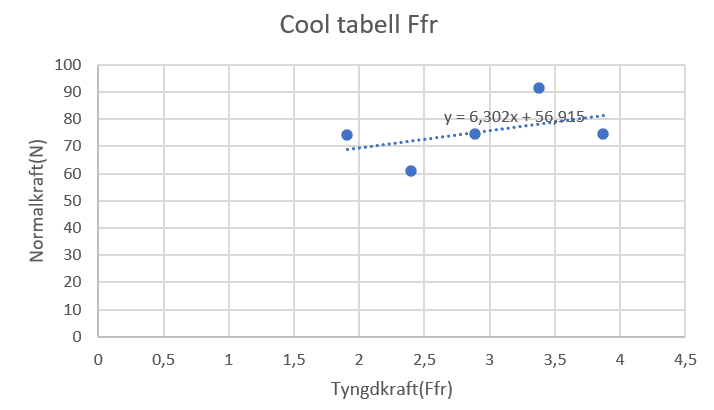
\includegraphics[width=0.8\textwidth]{images/tabell fysik labb2.PNG}
            \caption{En bild som visar de slutgiltiga mätvärdena i punktform i ett diagram, trendlinjen visar även dess funktion.}
            \label{fig:lutandeplan}
        \end{figure}
        
        Med brädan som triangels hypotenusa så blev höjden på våran triangel lika med höjden som det krävdes för att klossen skulle glida ned.
    \newpage
	\section{Analys och beräkning}
        Datat från beräkningarna visas i en tabell, den första tabellen visar tyngdkraften och normalkraften för träblocket
        och den andra tabellen visar hur vikten påvärkade längden på fjädern.\ref{table:result}



        \begin{table}
            \begin{center}
            \begin{tabular}{ |c|c| } 
                \hline
                Tyngdkraft (Ffr) & Normalkraft (N)  \\
                \hline
                1,907462 & 74,199762 \\
                2,397812 & 61,038768 \\
                2,888162 & 74,3909985 \\
                3,378512 & 91,558152 \\
                3,868862 & 74,3909985 \\

                \hline
            \end{tabular}
                \caption{Mätvärden}
                \label{table:result}
            \end{center}
        \end{table}

        \ref{table:result2}

        \begin{table}
            \begin{center}
                \begin{tabular}{ |c|c| }
                    \hline
                    Vikt (g) & Längd (cm)  \\
                    \hline
                    50 & 28 \\
                    100 & 35 \\
                    150 & 43 \\
                    200 & 51 \\
                    250 & 58 \\

                    \hline
                \end{tabular}
                \caption{Mätvärden}
                \label{table:result2}
            \end{center}

                \end{table}





    Datat importeras i Excel och alla mätvärden beräknas med hjälp av formler.
    \begin{equation}
        v_m = \frac{\Delta s}{\Delta t}
    \end{equation}
    
    \section{Slutsats och resultat}
        Längdvärdena beroende på när klossen gled ned för triangeln stoppas in som en tabell i excel.
        Med dessa värden kan sinus a beräknas i triangeln vilket sedan ger cosinus a och basen på triangeln.
        Tyngdkraften räknas ut genom att ta gravitationen(9,807 N) och gångrar det med klossens vikt i kg. Normalkraften
        räknas ut genom att ta arccos på triangeln och gångra med tyngdkraft och gravitationen:
        cos a = b/c, arccos a = -cos(cos a),
        Normalkraft(N) = arccos a * Ffr * 9,807


        Resultatet av beräkningarna illustreras i grafen och tabellerna ovan.
    \section{Diskussion} 
    Resultaten kan verka lite konstiga då höjden som brädan krävde för att klossen skull glida ned
    fluktuerade upp och ned över när vikt sattes på klossen. Detta är därför att vi bara mätte med ögat och linjal.
    Detta ger då inte ett exakt värde och vi kan ha sett fel.

    
    \printbibliography

\end{document}

